\section{Relay Attack on Intel SGX}

Trusted execution environments (TEEs) like Intel's SGX enable to securely execute applications on untrusted computing platforms. Remote attestation is a key feature of SGX, and other similar TEE architectures, as it allows a remote verifier to check that the attested enclave was correctly constructed before provisioning secrets to it. 

\begin{figure}[t]
 \centering
  %\includegraphics[trim={0 13.4cm 11cm 0},clip,width=\linewidth]{relayAttack.pdf}
  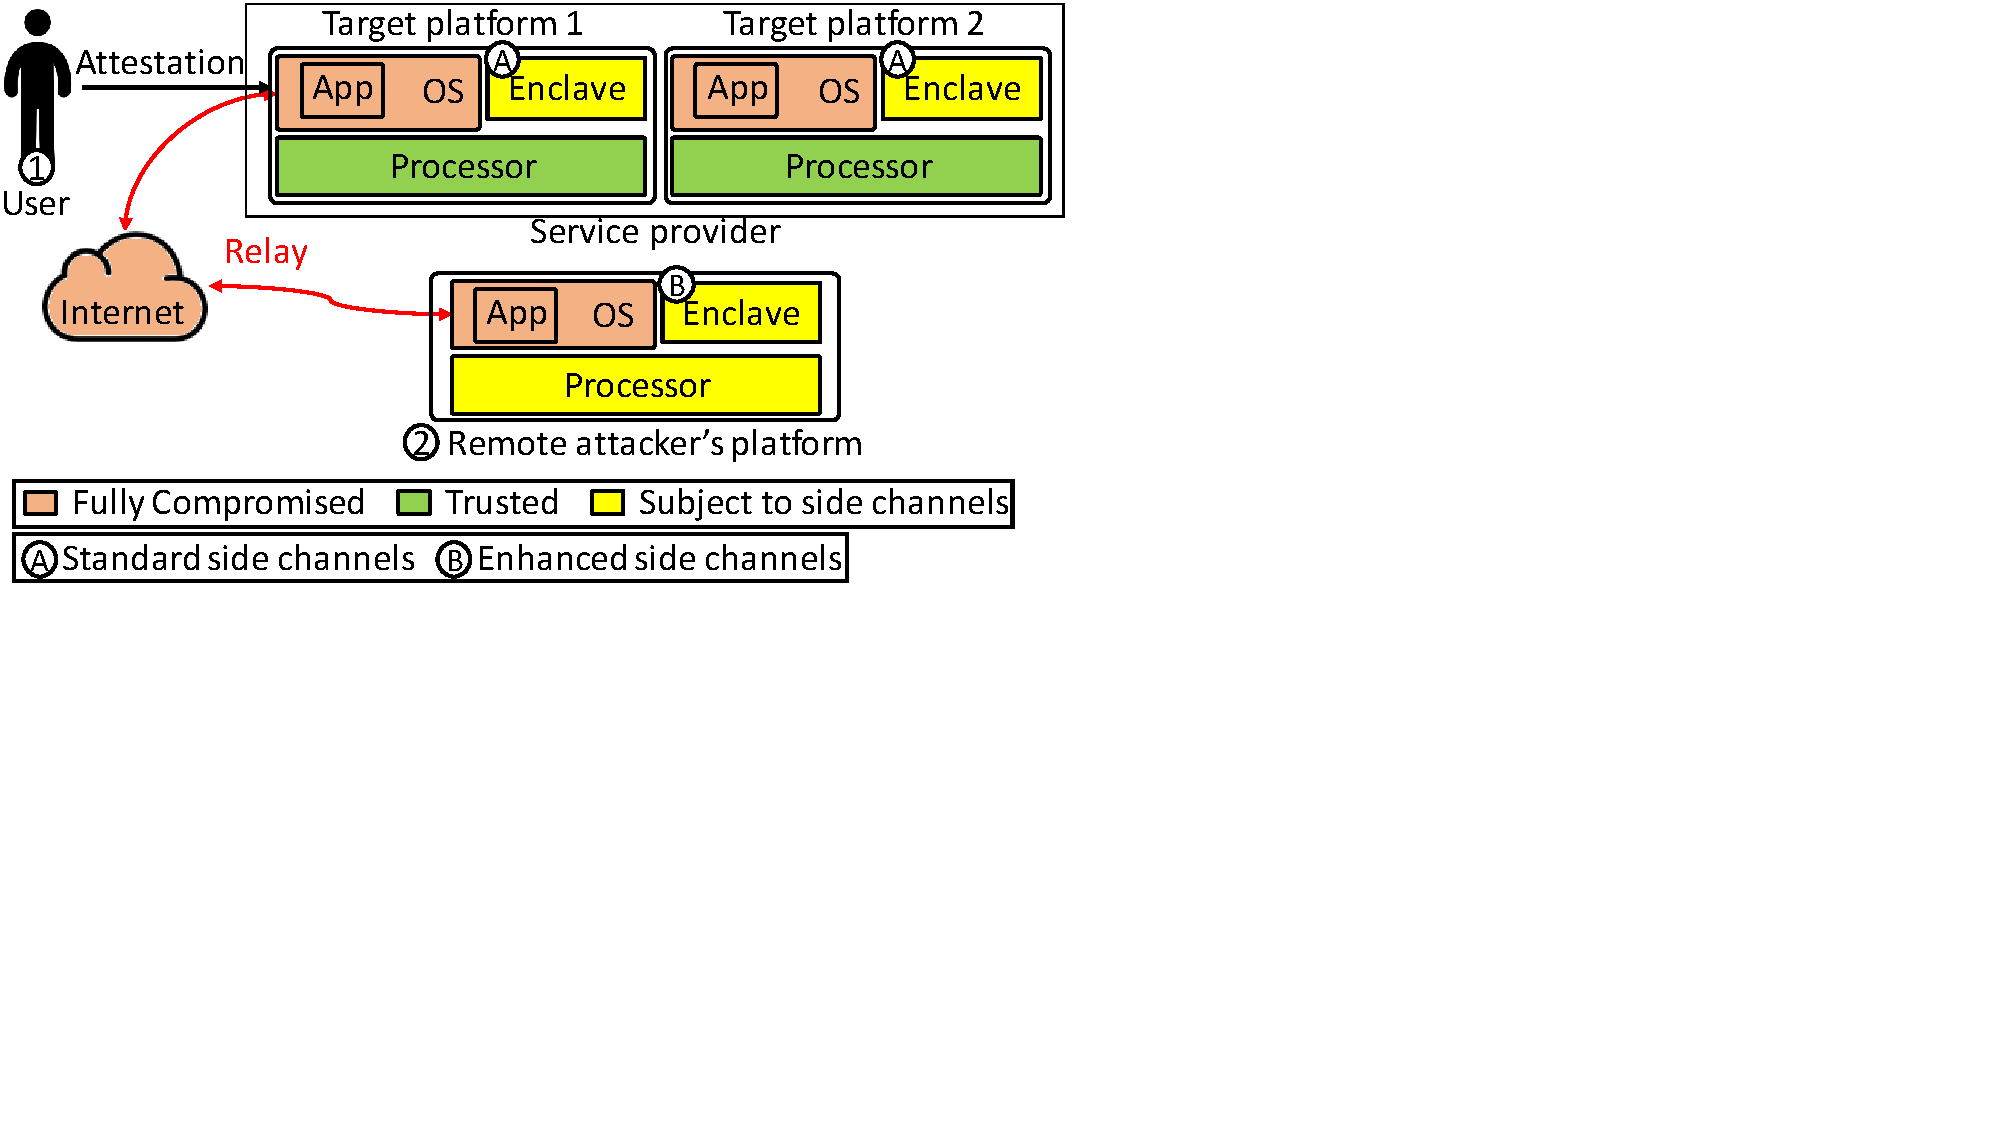
\includegraphics[trim={0cm 9cm 15.8cm 0},clip,width=0.75\linewidth]{relayAttack2.pdf}
 \caption{\textbf{Relay attack.} The adversary redirects attestation to his own platform which gives him increased (side-channel and kernel-level) abilities to attack the attested enclave.}
 \label{fig:SystemModel}
\end{figure}

\subsection{Relay Attacks}

We consider a system model shown in Figure~\ref{fig:SystemModel} that consists of three parties: the target platform, the remote verifier, and the attacker's platform. The remote verifier is a trusted party that wishes to connect and attest to a specific SGX platform. The target platform is the SGX platform to which the remote verifier intends to connect. Finally, the attacker's platform is a platform owned by the attacker that is connected to the target platform through the Internet.

\myparagraph{Adversary model.} We consider the following adversary model that we call the \emph{relay attacker}. The relay attacker controls the OS and all other privileged software on the \emph{target} platform at least \emph{temporarily}, in particular at the time of the remote attestation. The OS compromise on the target platform may be later detected and disinfected. We consider the case in which the target platform resides in a data center or otherwise in a facility with restricted physical access. The attacker hence \emph{does not} have physical access to the target platform (or any other co-located platform in the same facility).

The relay attacker controls the OS and all other privileged software on the attacker's platform \emph{permanently} and has physical access to that platform. The attacker also controls the network between the target platform and his platform. At the time of the attestation, the adversary has not been able to extract attestation or sealing keys from his platform or any other SGX processor.

\myparagraph{The relay attack.} The relay attacker can redirect the attestation requests intended for the target platform to his platform, as shown in Figure~\ref{fig:SystemModel}. This is a realistic attack for two reasons. First, in the SGX attacker's model the adversary is allowed to control the OS and can hence easily redirect any network request the target platform receives. Second, even if the attacker cannot compromise the OS in the target platform, it might be able to exploit some vulnerability of the untrusted application managing the enclave. The exploit might allow the attacker to manipulate the application's control flow to redirect attestation request to any platform he desires.


\begin{figure}[t]
\footnotesize
    \centering
    \begin{tikzpicture}[
solved/.style={rectangle,draw,fill=purple!40, rounded corners, align=center},
not/.style={rectangle, draw,fill=orange!60, rounded corners, align=center},
neutral/.style={rectangle, draw, rounded corners, align=center, fill=black!5},
sibling distance=12em]]
    \node[neutral](root) {SGX attacks}
    child { node[not, yshift=13pt] (name) {Attacks enabled by \\ leaked attestation keys ~\cite{foreshadow-usenix18}} }
    child { node[neutral, yshift=13pt] (app) {Side-Channels \\ on application enclave}
      child { node[neutral, yshift=12pt] (soft) {Software/digital}
		child { node[solved, yshift=0pt] (pe) {Privilege\\ escalation}}      
        child { node[not, right=1.5em of pe] (a) {Case (A) in Figure~\ref{fig:timeLine}:\\Complement of Case (B)}}
        child { node[solved, right=1.5em of a, yshift=-2pt] {Case (B) in Figure~\ref{fig:timeLine}:\\
            \begin{tabular}{rl}
                Target platform:& secure\\
                Attacker's platform:& vulnerable\\
            \end{tabular}}} }
      child { node[solved, yshift=12pt] (physical) {Physical} } };
      
    %\node[below=0cm of name] {Foreshadow~\cite{foreshadow-usenix18}};
    \node[below=0cm of physical](power) {Power analysis~\cite{wang2006covert}};
    \node[below=-5pt of power](EM) {EM radiation~\cite{gandolfi2001electromagnetic}};
    \node[below=-5pt of EM](ac) {Acoustic~\cite{shamir2004acoustic}};
         
    \node[left=10pt of soft](page) {Page fault~\cite{xu2015controlled}};
    \node[above=-3pt of page](cache) {Cache~\cite{dall2018cachequote}};
    \node[below=-2pt of page](branch) {Branch prediction~\cite{lee2017inferring}};
    %\node[below=-5pt of branch](synch) {Synchronization~\cite{asyncshock}};
      
    \node[solved, right=4em of root,  minimum size=3mm](l1) {};
    \node[right=0cm of l1](l1_1) {Enabled by relay};
    \node[not, below=1pt of l1, minimum size=3mm](l2) {};
    \node[right=0cm of l2](l2_1) {Independent of relay};
    
    \end{tikzpicture}
    
    \caption{\textbf{Relay attack implications.} The tree shows the types of attacks that are enabled by  redirection and ones that are independent of relay.}
    \label{fig:relayTree}
\end{figure}

            
\subsection{Relay Attack Implications}
\label{sec:problemStatement:implication}

Although relay attacks have been known for a long time~\cite{parno2008bootstrapping}, their implications to modern TEEs like SGX have not been carefully analyzed. Next, we perform the first such analysis.

The main consequence of attestation redirection is that it \emph{increases the adversary's ability to attack the attested enclave} through side-channels which are a well-known limitation of SGX (see Section~\ref{sec:background:attacks}). In Figure~\ref{fig:relayTree} we highlight two major classes of attacks: those that are only possible by first performing a relay attack, which we denote as ``enabled by relay'', and those that can be done whether or not the attacker also does a relay attack, which we call ``independent of relay.''

\myparagraph{Attacks using leaked attestation keys.}
Our first observation is that attacks based on leaked attestation keys (e.g., ones obtained through the Foreshadow attack~\cite{foreshadow-usenix18}) are independent of relaying. If the adversary has obtained a valid and non-revoked attestation key, he can emulate an SGX processor on the target platform and obtain any secrets provisioned to it. %We revisit such emulation attacks and propose a solution for addressing them in Appendix~\ref{sec:variantII}. 

\myparagraph{Physical side channels.}
One major benefit of the relay, from the adversary's point of view, is that it enables \emph{physical} side-channel attacks against application enclaves. Once a secret has been provisioned to the attacker's platform, she has as much time as she likes to perform the attack. Some examples of physical side-channel attacks are acoustic, electric and electromagnetic monitoring, which have been shown to be both effective and inexpensive means to extract secrets from modern PC platforms . Since the adversary does not have physical access to the target platform, such attacks are clearly not possible without relay. Hardening programs like enclaves against physical side channels is difficult and currently an open problem. Therefore, developers cannot easily defend their enclaves against physical side channels that are enabled by attestation redirection.

\myparagraph{Privilege escalation for digital side channels.}
Another possible benefit of relay attacks is that it may enable \emph{privilege escalation}. In cases where the adversary has only compromised the user-space application that manages the enclave, and not the OS, the application can redirect the attestation to the attacker's remote platform where he controls the OS as well. In such cases, the relay enables \emph{digital} side-channel attacks that require system privileges.

\iffalse
\begin{figure}[t]
\footnotesize
    \centering
    \begin{tikzpicture}[
    solved/.style={rectangle,draw,fill=purple!40, rounded corners, align=center},
    relayNode/.style={circle,draw,fill=red!40, align=center},
    edge from parent/.style={draw,-latex},    
    neutral/.style={rectangle, draw, rounded corners, align=center, fill=black!5},
    not/.style={rectangle, draw,fill=orange!60, rounded corners, align=center},
    sibling distance=12em]]
    
        
  \node[neutral](root1) {OS compromised}
        child { node[neutral, below = 1em of root1] (attestation1) {Attest enclave}     
         child { node[relayNode, right = 1em of attestation1] (relay1) {Relay}}
            child { node[neutral, below = 1em of attestation1] (discovery1) {New attack discovery}
                child { node[neutral, below = 1em of discovery1] (provisioning1) {Secret provisioning}     
                        child { node[neutral, below = 1em of provisioning1] (cleanup1) {OS cleanup} 
                            child { node[not, below = 1em of cleanup1] (attack1) {Independent of relay}  } } } } };  
            
   \node[below=0cm of attack1] {Case (A)};
 
 
  \node[neutral, right = 9em of root1](root) {OS compromised}
        child { node[neutral, below = 1em of root] (attestation) {Attest enclave}     
         child { node[relayNode, right = 1em of attestation] (relay) {Relay}}
             child { node[neutral, below = 1em of attestation] (provisioning) {Secret provisioning} 
                child { node[neutral, below = 1em of provisioning] (cleanup) {OS cleanup}
                child { node[neutral, below = 1em of cleanup] (discovery) {New attack discovery}                 
                            child { node[solved, below = 1em of discovery] (attack) {Enabled by relay}  } } } } };  
                
    \node[below=0cm of attack] {Case (B)};
    
    
    \end{tikzpicture}
    \caption{Example sequences of events where attestation redirection either enables digital side-channel attacks (B) or where the attack success is independent of relay (A). \todo{This figure should be improved. Where is the secret provisioned and at which time is all that matters. But this info is not clearly conveyed in the picture.}} 
    \figsaver
    \label{fig:timeLine}
\end{figure}
\fi

\begin{figure}[t]
\footnotesize
    \centering
    \begin{tikzpicture}[
    solved/.style={rectangle,draw,fill=purple!40, rounded corners, align=center},
    relayNode/.style={circle,draw,fill=red!40, align=center},
    edge from parent/.style={draw,-latex},    
    neutral/.style={rectangle, draw, rounded corners, align=center, fill=black!5},
    not/.style={rectangle, draw,fill=orange!60, rounded corners, align=center},
    sibling distance=12em]]
    
 
 
 \node[] (targetA) {\textbf{Target}};
 \node[right=0.93cm of targetA] (attackA) {\textbf{Attacker}};
 \node[below=0 of attackA] (dummy) {};
 
  
 \node[neutral, below=0.1cm of targetA](root1) {OS compromised};    
 \node[relayNode, below = 1em of root1] (relay1) {Relay};
 \node[neutral, right = 3em of relay1] (attestation1) {Attest enclave};
 \node[neutral, below = 1em of relay1] (discovery1) {New attack\\ discovery};        
  \node[neutral, below = 2.2em of attestation1] (discoveryAttack1) {New attack\\ discovery};  
 \node[neutral, below = 0.6em of discoveryAttack1] (provisioning1) {Secret\\ provisioning};
 \node[neutral, below = 3.5em of discovery1] (cleanup1) {OS cleanup};    
 \node[below = 3em of cleanup1] (end) {};      
 \node[not, below = 2em of provisioning1] (independent) {Independent of relay}; 
 
 
  \draw[->, thick] (root1) edge[] node{} (relay1);
 \draw[->, thick] (relay1) edge[] node{} (discovery1);
 \draw[->, thick] (relay1) edge[] node{} (attestation1);
 \draw[->, thick] (attestation1) edge[] node{} (discoveryAttack1);
 \draw[->, thick] (discovery1) edge[] node{} (cleanup1); 
 \draw[->, thick] (discoveryAttack1) edge[] node{} (provisioning1);
 \draw[->, thick] (provisioning1) edge[] node{} (independent);
 \draw[->, thick] (dummy) edge[] node{} (attestation1);
 \draw[->, thick] (cleanup1) edge[] node{} (end);
  \node[below=0cm of independent] {Case (A)};
 

 \node[right=0.52cm of attackA](point1){};
 \node[below=19em of point1](point2){Time};
 \draw[->] (point1) edge[] node{} (point2);
 
 \node[right=1.2cm of attackA] (targetB) {\textbf{Target}};
 \node[right=1.05cm of targetB] (attackB) {\textbf{Attacker}};
  \node[below=0 of attackB] (dummy1) {};
 
 %\draw ($(attackA)!0.5!(targetB)$) -- ($(attackA)!0.5!(targetB) - (0, 5)$);    
 \node[neutral, below=0.1cm of targetB](root) {OS compromised};
 \node[relayNode, below = 1em of root] (relay) {Relay};
 \node[neutral, right = 3.5em of relay] (attestation) {Attest enclave};
 \node[neutral, below = 0.6em of attestation] (provisioning) {Secret\\ provisioning};
 \node[neutral, below = 2em of relay] (cleanup) {OS cleanup};
 \node[neutral, below = 1em of cleanup] (discovery) {New attack\\ discovery};   
 \node[below = 3.5em of discovery] (end1) {};        
 \node[neutral, below = 2.5em of provisioning] (discoveryAttack) {New attack\\ discovery};           
 \node[solved, below = 1.7em of discoveryAttack] (attack) {Enabled by relay}; 
 
 
 \draw[->, thick] (root) edge[] node{} (relay);
 \draw[->, thick] (cleanup) edge[] node{} (discovery); 
 \draw[->, thick] (discoveryAttack) edge[] node{} (attack);
 \draw[->, thick] (relay) edge[] node{} (cleanup);  
 \draw[->, thick] (provisioning) edge[] node{} (discoveryAttack); 
 \draw[->, thick] (relay) edge[] node{} (attestation);
 \draw[->, thick] (attestation) edge[] node{} (provisioning);        
 \draw[->, thick] (dummy1) edge[] node{} (attestation);
 \draw[->, thick] (discovery) edge[] node{} (end1);
\node[below=0cm of attack] {Case (B)};
   

                         
    \end{tikzpicture}
    \caption{Example sequences of events. In Case A the attack success is independent of relay. In Case B attestation redirection enables the attack.} 
    \figsaverL
    \label{fig:timeLine}
\end{figure}


\myparagraph{Attacks that depend on timing of events.}    
The third, and perhaps the most subtle, implication of relay is that it can also enable software-based side-channel attacks that would not be possible to launch on the target platform due to \emph{timing of certain events}. These events include, but are not restricted to the provisioning of secrets to the enclave, the possible disinfection of the target platform from malicious software, and the discovery of a new side-channel attack. 

We group the relative ordering of these events into two cases: A and B. Case A covers event sequences that only lead to attacks which are independent of relay and Case B covers event sequences in which redirection gives extra capabilities to the adversary. Below, and in Figure~\ref{fig:timeLine}, we provide examples of sequences belonging to these two cases:

\begin{mylist}
    \item[\emph{Case A: independent of relay.}] A digital side-channel is independent of relay if the adversary could perform it on the target platform as well. An example of such case is shown th timeline depicted in Figure~\ref{fig:timeLine}, where a new attack is discovered after secret provisioning but before the target platform OS is disinfected.
    
    %If the vulnerability was discovered before the secret provisioning, we could assume that the enclave developers patched these vulnerabilities in the code. Hence attacker cannot execute the side channel attack after the relay. However, in case the developers did not publish the patched version of the enclave code before the provisioning of the secret to the enclave, the attacker can still execute relay attack and the extract the secret from his platform.

    \item[\emph{Case B: attack enabled by relay.}] Case B is reached whenever it occurs that by using a side channel the enclave is exploitable on the attacker's platform, but not on the target platform. 
    %In this case, by having the foresight to provision the enclave on its platform, the attacker has the possibility to launch an attack on an enclave that would otherwise be secure on the target platform. 
    A timeline of such case is shown in Figure~\ref{fig:timeLine}, where at the time of attestation and secret provisioning, the enclave is hardened against all known digital side-channel attacks (using tools like Raccoon~\cite{raccoon}). After secret provisioning, the OS compromise is detected and cleaned. Later, a new side-channel attack vector (that is not prevented by the used tools) is discovered. If the adversary performed redirection and the secret was provisioned to the attacker's machine, the new side channel is exploitable. Without the relay, the attack is not possible.
    
    %If the vulnerability is discovered after the secret provisioning, that attacker will have some time on this platform (relayed) where the unpatched enclave code runs before the software patch takes place.} 
\end{mylist}